% !TEX encoding = UTF-8 Unicode
%%%%%%%%%%%%%%%%%%%%%%%%%%%%%%%%%%%%%%%%%
% Simple Sectioned Essay Template
% LaTeX Template
%
% This template has been downloaded from:
% http://www.latextemplates.com
%
% Note:
% The \lipsum[#] commands throughout this template generate dummy text
% to fill the template out. These commands should all be removed when 
% writing essay content.
%
%%%%%%%%%%%%%%%%%%%%%%%%%%%%%%%%%%%%%%%%%

%----------------------------------------------------------------------------------------
%	PACKAGES AND OTHER DOCUMENT CONFIGURATIONS
%----------------------------------------------------------------------------------------

\documentclass[12pt]{article} % Default font size is 12pt, it can be changed here

\usepackage{geometry} % Required to change the page size to A4
\geometry{a4paper} % Set the page size to be A4 as opposed to the default US Letter

\usepackage{graphicx} % Required for including pictures

\usepackage{float} % Allows putting an [H] in \begin{figure} to specify the exact location of the figure
\usepackage{wrapfig} % Allows in-line images such as the example fish picture

\usepackage{lipsum} % Used for inserting dummy 'Lorem ipsum' text into the template

\linespread{1.2} % Line spacing

%\setlength\parindent{0pt} % Uncomment to remove all indentation from paragraphs

\graphicspath{{Pictures/}} % Specifies the directory where pictures are stored

\usepackage{listings}
\usepackage[spanish]{babel}
\selectlanguage{spanish}
\usepackage[utf8]{inputenc}
\usepackage{hyperref}
\begin{document}

%----------------------------------------------------------------------------------------
%	TITLE PAGE
%----------------------------------------------------------------------------------------

\begin{titlepage}

\newcommand{\HRule}{\rule{\linewidth}{0.5mm}} % Defines a new command for the horizontal lines, change thickness here

\center % Center everything on the page

\textsc{\LARGE Universidad de Salamanca}\\[1.5cm] % Name of your university/college
\textsc{\Large Administración de Sistemas}\\[0.5cm] % Major heading such as course name
%\textsc{\large Minor Heading}\\[0.5cm] % Minor heading such as course title

\HRule \\[0.4cm]
{ \huge \bfseries Python}\\[0.4cm] % Title of your document
\HRule \\[1.5cm]

\begin{minipage}{0.4\textwidth}
\begin{flushleft} \large
\emph{Autor:}\\
Diego \textsc{Martín} % Your name
\end{flushleft}
\end{minipage}
~
\begin{minipage}{0.4\textwidth}
\begin{flushright} \large
\emph{Profesora:} \\
Dr. Vivian \textsc{López} % Supervisor's Name
\end{flushright}
\end{minipage}\\[4cm]

%% Spanish!
{\large \today}\\[3cm] % Date, change the \today to a set date if you want to be precise

%\includegraphics{Logo}\\[1cm] % Include a department/university logo - this will require the graphicx package

\vfill % Fill the rest of the page with whitespace

\end{titlepage}

%----------------------------------------------------------------------------------------
%	TABLE OF CONTENTS
%----------------------------------------------------------------------------------------

\tableofcontents % Include a table of contents

\newpage % Begins the essay on a new page instead of on the same page as the table of contents 

%----------------------------------------------------------------------------------------
%	INTRODUCTION
%----------------------------------------------------------------------------------------

\large The Zen of Python\\
\small{Beautiful is better than ugly.\\
    Explicit is better than implicit.\\
    Simple is better than complex.\\
    Complex is better than complicated.\\
    Flat is better than nested.\\
    Sparse is better than dense.\\
    Readability counts.\\
    Special cases aren't special enough to break the rules.\\
    Although practicality beats purity.\\
    Errors should never pass silently.\\
    Unless explicitly silenced.\\
    In the face of ambiguity, refuse the temptation to guess.\\
    There should be one-- and preferably only one --obvious way to do it.\\
    Although that way may not be obvious at first unless you're Dutch.\\
    Now is better than never.\\
    Although never is often better than *right* now.\\
    If the implementation is hard to explain, it's a bad idea.\\
    If the implementation is easy to explain, it may be a good idea.\\
    Namespaces are one honking great idea -- let's do more of those!\\} 

\section{Introducción} % Major section

\subsection{\large ¿Por qué usar Python?}
	Para aquel que no aún no conozca las virtudes de este lenguaje, y qué ventajas proporciona para sus labores como programador, puede que al principio se muestre reacio a adoptar esta tecnología. Sin embargo, puede que estos principios de desarrollo hagan cambiar de opinión hasta al más acérrimo a otros lenguajes.
	\begin{itemize}
		\item Python es legible y coherente.\\
			`Legible, por tanto mantenible', es una de las premisas del lenguaje. Se aleja de lenguajes como Perl en ese aspecto. Además es un lenguaje orientado a objetos, lo cual aumenta su reusabilidad enormemente.\\
			Muchos dicen que Python \textit{encaja en tu cerebro}. Todo es comprensible cuando se dominan unos pocos conceptos clave. Además, el enfoque general es muy minimalista.
		\item Potenciar la productividad del programador\\
			Un código en Python ocupa 1/5 de su equivalente en C o Java. Además se elimina el proceso de compilación, dado que es un lenguaje interpretado\footnote{A lo largo de la historia del desarrollo de software se han dado situaciones en las que era difícil encontrar suficientes programadores para implementar ciertas aplicaciones. Actualmente los equipos se ven forzados a conseguir las mismas tareas con menos gente. En ambos escenarios, Python permite conseguir más con menos.}.
		\item Portabilidad\\
			Todos los programas en Python son multiplataforma \textit{per se} o requieren muy pocos cambios para trasladar un programa a otro sistema. Esto se aplica también a las interfaces gráficas de usuario.
		\item Bibliotecas de soporte\\
			Python cuenta con una gran cantidad de recursos de serie, permitiendo conseguir tareas de nivel de aplicación con la funcionalidad con la que se cuenta desde el momento en el que se instala. Además, existe una gran cantidad de código desarrollado por terceros y la posibilidad de crear módulos personales para solucionar tareas.
		\item Integración\\
			Python se integra con lenguajes y tecnologías como C, C++, Java, COM, Corba, .NET, SOAM, XML-RPC
		\item Disfrútalo\\
			Python es un lenguaje pensado para hacer al programador la tarea de desarrollar software mucho más amigable y entretenida.
	\end{itemize}
		
%------------------------------------------------

\subsection{Contras} % Sub-section

El principal problema de Python es su rendimiento. Al ser un lenguaje interpretado y no compilado, no es tan potente como C o C++. Sin embargo actualmente se ha mejorado notablemente su rendimiento gracias a la traducción del código a un \textit{bytecode}, que es realmente el conjunto de sentencias utilizado por la PVM (Python Virtual Machine).
Generalmente es un lenguaje rápido, y cuando es necesario optimizar el rendimiento al máximo, se puede realizar una traducción a C y traducirlo posteriormente a código máquina, por lo que se ejecutaría a velocidades nativas. También es posible escribir estas partes directamente en C y enlazarlas al resto del código.

%------------------------------------------------

\subsection{¿Quién usa Python?} % Sub-section

Con un número de usuarios entre 500,000 y un millón de usuarios, Python cuenta con una comunidad muy grande. Compañías como Google o Yahoo! utilizan el lenguaje en sus servicios en red, y para HP, Seagate o IBM es una herramienta de utilidad a la hora de realizar pruebas de hardware\footnote{La lista completa se puede encontrar en \href{http://www.python.org}{python.org}}
Proyectos como el microordenador Raspberry Pi promocionan y utilizan Python como lenguaje principal de programación a la hora de enseñar a nuevos programadores y al utilizar el dispositivo.
%%Raspberry
%%------------------------------------------------
%
%\subsubsection{Subsubsection 1} % Sub-sub-section
%
%\lipsum[3] % Dummy text
%
%\begin{figure}[H] % Example image
%\center{
\includegraphics[width=0.5\linewidth]{placeholder}}
%\caption{Example image.}
%\label{fig:speciation}
%\end{figure}
%
%%------------------------------------------------

%\subsubsection{Subsubsection 2} % Sub-sub-section
%
%\lipsum[4] % Dummy text

\subsection{¿Qué se hace con Python?}
\begin{description}
	\item[Administración de sistemas]
	Crear interfaces para servicios de un sistema operativo es muy sencillo en Python, lo cual lo convierte en una herramienta idónea para administradores de sistemas a la hora de trabajar con árboles de directorios, búsqueda de ficheros, lanzamiento de otros programas, procesamiento paralelo \dots
	\item[Interfaces Gráficas de Usuario]
	Crear interfaces en Python es muy simple. El entorno trabaja de forma natural con objetos diseñados para crear IGUs, como Tk Tkinter, que se adapta a la estética de cada plataforma, wxPython, basada en C++ o PythonCard.
	\item[Scripting]
	Es fácil realizar tareas de red con Python, y es muy utilizado para CGI(\textit{Common Gateway Interface}), FTP, sockets o HTML. Módulos como HTMLGen permiten generar código y otros como win32all insertan código Python como JavaScript. Además, utilizades como Zope, WebWare o Quixote permiten el desarrollo de sitios web grandes de forma rápida y sencilla.
	\item[Prototipado]
	Debido a que el desarrollo en Python es muy ágil, muchos desarrolladores aprovechan esta característica para generar `esbozos' de sus proyectos para evaluarlos antes de crear la versión definitiva en otro lenguaje. Aprovechando además la integración con otros lenguajes, en ocasiones partes del prototipo en Python son integradas en el resto del código.
	\item[Programación numérica, juegos, trabajo con imágenes, inteligencia artificial, etcétera]
	%%Revisar
\end{description}

\subsection{Fortalezas técnicas de Python}
\begin{itemize}
	\item Es un lenguaje orientado a objetos.
	\item Es libre (licencia de la Python Software Foundation, compatible con la GPL).
	\item Muy soportado.
	\item Espíritu de comunidad.
		Guido van Rossum, creador de Python es el \textit{Benevolent Dictator For Life of Python} (Benevolente dictador vitalicio de Python, orquesta a un equipo de 1000 personas encargados de mejorar el lenguaje. Los cambios siguen un proceso de mejora formal, que es analizado por Guido. Esta metodología hace que el desarrollo sea mucho más conservador que en otros lenguajes.
	\item Portabilidad
	\item Potencia
		\subitem Es un lenguaje dinámicamente tipado.
		\subitem Gestión automática de la memoria, utilizando un contador de referencias
		\subitem Tipos predefinidos que cubren la mayoría de las estructuras de datos utilizadas.
		\subitem Gran variedad de herramientas incluidas en el lenguaje.
		\subitem Gran cantidad de bibliotecas y código de terceros
	\item Se combina con facilidad con otros lenguajes
	\item Es fácil de utilizar y aprender.
	\item Sintaxis clara.
\end{itemize}
%----------------------------------------------------------------------------------------
%	MAJOR SECTION 1
%----------------------------------------------------------------------------------------

\subsection{¿Cómo se ejecuta un programa en Python?} % Major section

Para ejecutar un programa en Python es necesario únicamente un intérprete y una biblioteca de soporte. El código es compilado a \textit{bytecode}, un código de bajo nivel e independiente de la plataforma utilizada. Un archivo .pyc es generado, y es interpretado por la máquina virtual de Python del sistema\footnote{Hay varias implementaciones de la máquina virtual: CPython está escrita en ANSI C, Jython, que cuenta con clases de Java que compilan el código de Python a \textit{bytecode} de Java, dirigiéndolo a la \textit{Java Virtual Machine} del sistema o Python.NET, que se integra con C\#.}.
Existen además implementaciones especiales, como JIT Python, que incorpora un compilador \textit{Just In Time}, o binarios `congelados' (\textit{frozen binaries}), que empaquetan todo lo necesario para que un programa se ejecute (máquina virtual, código, etcétera).

En todo código se deberá indicar la ruta del intérprete. Utilizando el fichero \verb+/usr/bin/env python+ obtenemos la ruta se encuentre donde se encuentre el intérprete, por lo que evitamos modificar el código a la hora de cambiar de sistema.
	\lstset{language=python, showspaces=false}
	\begin{lstlisting}[frame=single, showspaces=false]
	#!/usr/bin/env python
	\end{lstlisting}

También es posible trabajar directamente con la línea de comandos, y el lenguaje es compatible con tuberías y redirección de las diferentes entradas y salidas.

%%------------------------------------------------
%
%\subsection{Subsection 1} % Sub-section
%
%\subsubsection{Subsubsection 1} % Sub-sub-section
%
%\lipsum[6] % Dummy text
%
%%------------------------------------------------
%
%\subsubsection{Subsubsection 2} % Sub-sub-section
%
%\lipsum[6] % Dummy text
%\begin{wrapfigure}{l}{0.4\textwidth} % Inline image example
%  \begin{center}
%    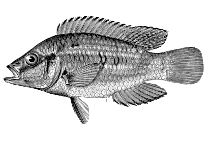
\includegraphics[width=0.38\textwidth]{fish}
%  \end{center}
%  \caption{Fish}
%\end{wrapfigure}
%\lipsum[7-8] % Dummy text
%
%%------------------------------------------------
%
%\subsubsection{Subsubsection 3} % Sub-sub-section
%
%\begin{description} % Numbered list example
%
%\item[First] \hfill \\
%\lipsum[9] % Dummy text
%
%\item[Second] \hfill \\
%\lipsum[10] % Dummy text
%
%\item[Third] \hfill \\
%\lipsum[11] % Dummy text
%
%\end{description} 

%----------------------------------------------------------------------------------------
%	MAJOR SECTION X - TEMPLATE - UNCOMMENT AND FILL IN
%----------------------------------------------------------------------------------------

%\section{Content Section}

%\subsection{Subsection 1} % Sub-section

% Content

%------------------------------------------------

%\subsection{Subsection 2} % Sub-section

% Content

%----------------------------------------------------------------------------------------
%	CONCLUSION
%----------------------------------------------------------------------------------------

\section{Números}

Trabajar con valores numéricos algo habitual en, si no la totalidad de las aplicaciones en cualquier lenguaje, en una inmensa mayoría. Python incorpora tipos predefinidos para simplificar las tareas más habituales.
Tipos de números:
\begin{itemize}
	\item Enteros (\verb+int+)
	\item Real en coma flotante (\verb+float+) y de doble precisión (\verb+float+)
	\item Como diferencia con otros lenguajes, Python soporta de forma nativa operaciones con números complejos.
\end{itemize}
El límite de tamaño para un número en Python lo determina la memoria, y debido al carácter dinámico del lenguaje, no es necesario definir el tipo de número. Operaciones con octales y hexadecimales son triviales también. La conversión es automática y se realiza siempre (a menos q	ue se especifique de forma explícita).
La representación es variable, utilizándose las funciones \verb+str()+ y \verb+repr()+ para cambiar de la forma utilizada por el ordenador a una representación más `humana'.

Los operadores de C han sido integrados en Python respetando la precedencia de cada uno. Se incluyen algunas novedades y mejoras en algunos operadores. Destacan:
\begin{itemize}
	\item Creación de funciones sin nombre (`anónimas'): \verb+lambda <argumentos>: <expresión>+
	\item \verb+is+ para determinar el tipo de objeto.
	\item Operador // para división con truncado.
	\item oct(), hex(), str(), repr\dots para conversiones de tipo.
	\item Nuevas operaciones con arrays y otras colecciones de datos (se verán más tarde)
\end{itemize}

\subsection{¿Cómo se almacena un elemento en memoria?}

Aprovechando que hemos cubierto el primer grupo de tipos de datos, es importante conocer cómo funciona una variable declarada en Python. Toda variable almacena una referencia a un elemento en memoria, por lo que las mismas no tienen un tipo definido. Esto no significa que los elementos en memoria no tengan tipos definidos. Al contrario, es importante conocer las características de cada uno, dado que la conversión entre tipos no es automática. Funciones como str() permiten realizar la transformación.
El contador de referencias es el encargado de la gestión de la memoria, liberando el espacio ocupado por un bloque de datos cuando se pierde la última referencia.
\section{Cadenas de texto}

Una cadena de texto en Python es un tipo especial de secuencia (las veremos posteriormente). No existe el tipo \verb+char+ como en C y, a diferencia de este, Python cuenta con un potente conjunto de utilidades para manipular cadenas.
Las cadenas de texto son elementos inmutables, por lo que una vez creados no se podrán modificar (es necesario crear una nueva cadena con los cambios si se desea alterar uno de estos elementos).
Ejemplos de literales \verb+string+:
\begin{itemize}
	\item Cadena vacía: \verb+cadena = ''+
	\item Cadena vacía (con dobles comillas): \verb+cadena = ""+
	\item Bloque vacío (un bloque permite representar cadenas de texto de varias líneas): \verb+bloque = """..."""+
	\item Cadena en bruto: \verb+bruto = r'\temp\haus'+
	\item Unicode: \verb+u'universal'+
	\item Formateo: \verb+"Resultados: %d" % resultados+
\end{itemize}

\subsection{Manipulación de cadenas}
{\Large Operadores}
\begin{itemize}
	\item Concatenación: \verb|+|
	\item Repetición: \verb+*+
	\item Índice: \verb+cadena[indice]+
	\item Longitud: \verb+len(cadena)+
	\item Búsqueda de elementos: \verb+cadena.find('Waldo')+
	\item Iteración: \verb+for x in cadena+
	\item Longitud: \verb+len()+
\end{itemize}

{\Large Métodos}
\begin{itemize}
%%Completar
	\item \verb+cadena.capitalize()+
	\item \verb+cadena.center()+
	\item \verb+.encode(), .endswith(), .expandtabs()+ \dots
	\item \verb+.isalnum(), .isdigit(), .istitle(), .isupper()+ \dots
\end{itemize}


El soporte de Unicode está integrado en el lenguaje, y siempre que se combinen con otros tipos de cadenas (por ejemplo, en una concatenación) el resultado será una cadena Unicode.
Dado que una cadena es un conjunto ordenado de caracteres pueden ser manipuladas mediante índices.

\subsection{Secuencias de escape}
\begin{itemize}
	\item \verb+\newline+
%completar
\end{itemize}

\subsection{Formateo avanzado de cadenas}
Se puede utilizar cualquier especificados de formato de C en Python, así como alguno nuevo.
\begin{itemize}
	\item \verb+%s+
	\item \verb+%d+
	\item \verb+%r+
\end{itemize}

\subsection{Consideraciones especiales}
Una cadena no se convierte automáticamente a número o a cualquier otro tipo de datos, es necesario hacerlo explícitamente.

\section{Listas y diccionarios}
Existen tres categorías generales en Python: números, secuencias y mapas. Cada una de ellas tiene unas propiedades especiales y operaciones asociadas a él. Hasta ahora hemos visto las dos primeras (números y secuencias, dado que las cadenas de caracteres son un tipo de estas). La categoría restante, los mapas.

Las listas son la colección de elementos ordenada más flexible de Python. Pueden contener cualquier elemento, dado que son meramente colecciones de referencias, y permiten anidar más listas dentro de ellas.
Una ventaja de Python es que la mayoría de las operaciones que en otros lenguajes deben ser implementadas por el programador se encuentran disponibles de serie en el lenguaje.
Las propiedades de estas soluciones son:
\begin{itemize}
	\item Son mutables, de longitud variable y orden definido.
	\item Se accede por índices.
	\item Colecciones de referencias. Obtener un elemento es tan rápido como en C (de hecho son arrays de C dentro del intérprete). Mientras que no se especifique explícitamente, los elementos son referencias y no copias.
\end{itemize}
Ejemplos de listas:
\begin{lstlisting}[frame=single, showspaces=false]
#!/usr/bin/env python
L1 = [];
L2 = ['abc', 'is', 'as', 'easy', 'as'];
L2.append('123');
\end{lstlisting}
Operaciones con listas:
\begin{itemize}
	\item Operaciones básicas: len(), \verb+['Monty'] *4+ (multiplicación).
	\item \verb+for x in [1,2,3]: print x+
	\item \verb#[1,2] + list("34")# \footnote{Importante, utilizar operadores con distintos tipos de operados generará un error.}.
	\item Modificación: \verb+.sort(), .extend()+
\end{itemize}
\subsection{Diccionarios}
Los diccionarios son el tipo más flexible que viene integrado en Python. Son colecciones sin orden de elementos, cuya distinción respecto las listas es que los elementos son de tipo valor-clave. Pertenecen a la categoría de mapas mutables, y se accede a ellos mediante una clave. No tienen un orden particular\footnote{De hecho, Python ordena aleatoriamente los elementos para conseguir un acceso más rápido}. Las claves son localizaciones simbólicas de ítems en un diccionario.
Son colecciones de longitud variable, heterogéneas y arbitrariamente anidables.
La sintaxis de sus elementos es \verb+{clave:valor}+. Ejemplos de diccionarios:
\begin{itemize}
	\item D={'spam':1, 'eggs':2};
	\item Operaciones: \verb+.copy(), .keys(), .has_key(), .values(), .get(clave, defecto)+
	\item Acceso a elementos: tal y como en un array: \verb+D['spam']+
	\item Concatenación: \verb+D.update(d1)+
\end{itemize}
Son muy utilizados como estructuras de datos para una multitud de casos.

\section{Tuplas, archivos y otras estructuras de datos}
Las tupas son colecciones equivalentes a las listas, pero de carácter inmutable. Declarar una tupla es muy parecido a la creación de listas:
\begin{lstlisting}[frame=single, showspaces=false]
#!/usr/bin/env python
() 
t0 = (0,);
t1 = (0, 'Ni', 1.2, 3);
\end{lstlisting}
\subsection{¿Para qué sirve tener tipos inmutables y mutables?}
La principal ventaja de contar con ambos tipos es la flexibilidad de unos y las ventajas que proporciona contar con la garantía de que un elemento no se va a poder modificar.
\begin{wrapfigure}{l}{0.4\textwidth} % Inline image example
  \begin{center}
  %%Corregir
    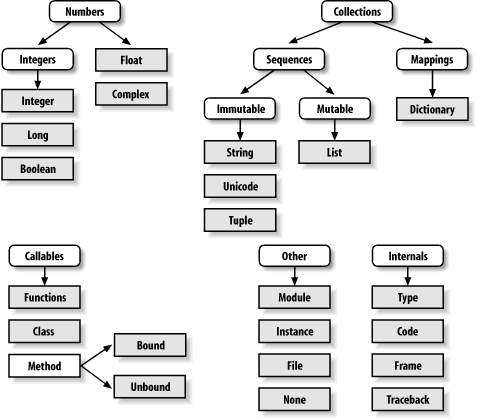
\includegraphics[width=0.7\textwidth]{tree.png}
  \end{center}
  \caption{Jerarquía de tipos predefinidos de Python.}
\end{wrapfigure}
\subsection{Índices. Las mejoras de Python}
Como hemos comentado a lo largo de este documento, Python incorpora mejoras al acceso a elementos en listas, tuplas y otro tipo de colecciones. Estos son nuevos operandos:
\begin{itemize}
	\item \verb+array[1:]+ : Retorna una lista con los elementos desde el 1.
	\item \verb+array[:4]+ : Retorna una lista con los elementos hasta el 4.
	\item \verb+array[1:3]+ :Lista con los elementos desde 1 a 3 (no inclusive)
	\item \verb+array[-1]+ : Último elemento
	\item \verb+array[:]+ : Todos los elementos del array
\end{itemize}
\subsection{Ficheros}
Para trabajar con un fichero es necesario almacenar en una variable un \textit{descriptor} del mismo. Existen las funcionen \verb+open()+, \verb+read()+ o \verb+write()+ para manipular archivos de forma sencilla, así como métodos más específicos, como \verb+readline()+


\section{Condicionales}
Un programa generalmente está compuesto por secuencias de control de flujo y repetición. En Python la primera categoría está protagonizada por la cláusula \verb+if+.
Ejemplo de una estructura condicional en Python:
\begin{lstlisting}[frame=single, showspaces=false]
if eggs:
	buy(1);
elif milk
	buy(6);
else:
	buy(0);
\end{lstlisting}
{\Large \textbf{Importante: no existe la sentencia} \verb+switch+}
Esta característica, que a muchos procedentes de lenguajes como Pascal o C no gustará, es fácilmente reemplazable por un diccionario:
\begin{lstlisting}[frame=single, showspaces=false]
elegir='jamon';
print{'leche': 1.25,
	'jamon':1.99,
	'huevos':0.99,
	'bacon':1.10}[elegir]
\end{lstlisting}
\subsection{Reglas de sintaxis}
\begin{itemize}
	\item Las sentencias se ejecutan una tras otra, a menos que se especifique lo contrario.
	\item Las sentencias y los bloques son detectados automáticamente: no se utilizan corchetes o cualquier otro tipo de delimitador. El indentado del código es lo que determina la pertenencia o no a un bloque.
	\item Líneas en blanco, espacios y comentarios son generalmente ignorados: especialmente en archivos. A la hora de trabajar con cadenas de caracteres se respetan. Los comentarios (marcados por un `\#' inicial) siempre son ignorados.
\end{itemize}

\section{Bucles}
While:
\begin{lstlisting}[frame=single, showspaces=false]
while x :
	print x,
	x = x[1:];
\end{lstlisting}
Herramientas de control: \verb+break+, \verb+continue+, \verb+pass+ y \verb+else+:
\verb+break+ y \verb+continue+ funcionan de la misma forma que en C, interrumpiendo el flujo del bucle más anidado e interrumpiendo la iteración que se da en ese momento para pasar a la siguiente respectivamente.
\verb+pass+ no hace nada. Es de utilidad cuando el lenguaje obliga al programador a incluir una sentencia en un bloque.
\verb+else+: Se ejecuta si y sólo si el bucle finaliza de forma normal (sin encontrarse con un \verb+break+).
Formato general de un bucle:
%%Revisar
\begin{lstlisting}[frame=single, showspaces=false]
while x :
	if x / 2 > 5:
		x=x+3
		break
	x--
else:
	print 'Error'
\end{lstlisting}
{\Large for:}
\begin{lstlisting}[frame=single, showspaces=false]
for x in [1,2,3]:
	print x
\end{lstlisting}

\section{Funciones}
Una función nos permite agrupar bloques de código a fin de separar componentes, reutilizarlos o invocarlos en varias ocasiones a lo largo del código. En Python contamos con las siguientes expresiones:
\begin{itemize}
	\item Llamadas: \verb+func("arg1", "arg")+
	\item Definición y retorno de elementos: \verb|def funcion(a, b): return a+b|
	\item Global: \verb+def funcion(): global x; x = 'nuevo'+
	\item Funciones lambda: \verb+funcs = [lambda x: x**2, lambda x: x*3]+
\end{itemize}

Para crear una función contamos con la sentencia \verb+def+. Esta sentencia no se ejecuta hasta que se alcanza en el flujo del programa, por lo que es completamente válido incluirla en cualquier punto del programa. Además, def genera un objeto que tiene un nombre asignado. Se convierte por tanto en una referencia a un objeto función. El operador \verb+return+ finaliza el flujo de la función y devuelve un objeto a quien invocó la función. Los argumentos son pasados como referencias. \verb+global+ declara variables a nivel de módulo que son asignadas. Por defecto, todos los nombres asignados en una función son locales a la misma y existen únicamente cuando la función se ejecuta. Utilizando \verb+global+ se permite ampliar el alcance del nombre definido.
Una función no se declara con un tipo de datos determinado, los argumentos, valores de retorno y variables pueden ser de cualquier tipo, lo cual aumenta la versatilidad de estos bloques de código.
También existen funciones anónimas con el operador \verb+lambda+.

\section{Módulos}
Los módulos de Python son piezas de código que permiten añadir herramientas a nuevos programas. A grandes rasgos constituyen paquetes de nombres, que son cargados o no en memoria según la funcionalidad que se desee aprovechar de los mismos, pudiendo seleccionar dentro de cada módulo qué componentes cargar.
Utilizar módulos es muy recomendable debido a que fomentan la reusabilidad del código, particionan el espacio de nombres e implementan servicios compartidos o datos (es posible que un sistema con distintas entidades que accedan a un conjunto común de datos cuente con una única copia de esta información gracias al uso de módulos).
Con la sentencia \verb+import+ añadimos un módulo al programa.
Python ya cuenta con un set de unos 200 módulos incluidos con la distribución general del lenguaje, que cubren las tareas más cotidianas.
\subsection{Creación de módulos}
Para definir un módulo se debe crear un código en Python, e importarlo a otro con las sentencias \verb+import+ o \verb+from+. Todo elemento en el nivel jerárquico superior es incluido a la lista de nombres del módulo y será accesible cuando se utilice el módulo. La diferencia entre ellos es que \verb+from+ permite seleccionar qué elementos importar, haciendo además que no sea necesario incluir el nombre del módulo cada vez que se desee utilizar un nombre.

\section{Clases, objetos y excepciones}
Como ya hemos dicho en numerosas ocasiones, Python es un lenguaje orientado a objetos. Una clase constituye una `plantilla' a partir de la cual crear una serie de objetos. Es importante tener en mente que la utilización de objetos en Python es completamente opcional, sin embargo es altamente recomendable utilizarlas, debido al potencial de este paradigma en el ámbito de la reutilización y aislamiento de código, la herencia y composición y la instanciación múltiple.
\subsection{Un ejemplo inicial}
\begin{lstlisting}[frame=single, showspaces=false]
class Perro:
	def Ladrar():
		print "Arrf"
	def Correr():
		print "Corriendo"
\end{lstlisting}
Para generar instanciaciones de estas clases utilizamos el nombre de la misma:
\begin{lstlisting}[frame=single, showspaces=false]
toby = Perro()
\end{lstlisting}

\subsection{Observaciones generales}
La orientación a objetos en Python contiene composición, herencia y interpretación de los operandos del lenguaje.
\subsection{Excepciones}
Las excepciones son mecanismos de control de situaciones irregulares dentro del flujo de un programa. Consisten en bloque de código rodeados por las palabras \verb+try+/\verb+except+ para capturar excepciones lanzadas por el lenguaje o por el usuario, \verb+try+/\verb+finally+ para operaciones finales tanto si se dan excepciones como si no, \verb+raise+ para lanzar excepciones manualmente en el código del usuario y \verb+assert+ como \textit{trigger} condicional para una excepción en el código del usuario del lenguaje. Generalmente son utilizadas para gestión de errores, notificaciones de eventos, manejo de situaciones especiales o acciones de finalización.
%\lipsum[12-13]

%%Documentation pg 171-Chapter 11
%----------------------------------------------------------------------------------------
%	BIBLIOGRAPHY
%----------------------------------------------------------------------------------------

%%Use
\begin{thebibliography}{99} % Bibliography - this is intentionally simple in this template

\bibitem[The Zen of Python, 2004]{Peters:2004dg}
Figueredo, A.~J. and Wolf, P. S.~A. (2009).
\newblock Assortative pairing and life history strategy - a cross-cultural
  study.
\newblock {\em Human Nature}, 20:317--330.
 
\end{thebibliography}

%----------------------------------------------------------------------------------------

\end{document}